\documentclass{beamer}
\input{praxis-beamer}

\usepackage{tikz}
\usetikzlibrary{positioning,calc}

\title{SPARK 2014 Advisory Panel}
\subtitle{Teleconference 1}

% Inspired by http://tex.stackexchange.com/questions/15237
\makeatletter
\newenvironment{btHighlight}[1][]
{\begingroup\tikzset{bt@Highlight@par/.style={#1}}\begin{lrbox}{\@tempboxa}}
{\end{lrbox}\bt@HL@box[bt@Highlight@par]{\@tempboxa}\endgroup}

\newcommand\btHL[1][]{%
  \begin{btHighlight}[#1]\bgroup\aftergroup\bt@HL@endenv%
}
\def\bt@HL@endenv{%
  \end{btHighlight}%
  \egroup
}
\newcommand{\bt@HL@box}[2][]{%
  \tikz[remember picture]{%
    \pgfpathrectangle{\pgfpoint{1pt}{0pt}}{\pgfpoint{\wd #2}{\ht #2}}%
    \pgfusepath{use as bounding box}%
    \node[anchor=base west,%
          outer sep=0pt,%
          inner xsep=1pt,%
          inner ysep=0pt,%
          rounded corners=2pt,%
          minimum height=\ht\strutbox+1pt,%
          #1]%
          {%
            \raisebox{1pt}{\strut}\strut\usebox{#2}%
          };%
  }%
}
\makeatother

\date{March 19, 2013}
\begin{document}

\begin{altrantitle}
\titleprismlabela{SPARK 2014}
\titleprismlabelb{High Assurance by Design}
\titleprismlabelc{
  \resizebox{4cm}{!}{
    
\includegraphics{partnership.pdf}
  }
}
\end{altrantitle}

\begin{frame}{Introduction}

  \begin{itemize}

  \item Introductions
  \item Progress update
  \item Round-up of LRM review comments
  \item Discussion Topics
  \item Conclusion

  \end{itemize}

  \end{frame}

\begin{frame}{Progress Update}

  \begin{itemize}

  \item Key active workstreams:
  
    \begin{itemize}
    \item SPARK 2014 Language Design
    \item GNAT front end
    \item Flow analyser
    \item Proof tools
    \end{itemize}

  \item Improved visualisation of errors ...

  \end{itemize}

\end{frame}

\begin{frame}[fragile]{Visualisation - Proof}

  \begin{itemize}

  \item Path display for failed verification conditions
  \item Example - failed array bounds check (line highlighted in red):
  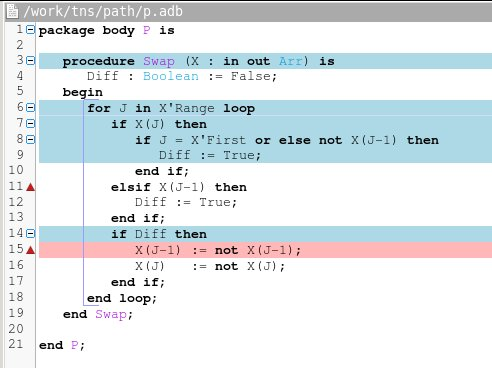
\includegraphics[width=0.5\textwidth]{show_path.jpg}
  \item Path (in blue) shows that we can have \verb|J = X'First|, so accessing the array at position \verb|J - 1| would be an error

  \end{itemize}

\end{frame}

\begin{frame}[fragile]{Visualisation - Flow Analysis}

  \lstdefinestyle{magic}{
    basicstyle=\tiny\tt,
    keywordstyle=\color{AnColour02},
    moredelim=**[is][{\btHL[fill=AnSecondaryRed!50,name=error]}]{`}{`},
    moredelim=**[is][{\btHL[fill=AnSecondaryYellow!50]}]{@}{@},
  }

  The new flow analysis allows for \structure{better error
    explanations} using program slices.

  \vskip 0.5cm

  \begin{onlyenv}<1>
  \begin{pxcode}[language=SPARK,style=magic,gobble=4]
    procedure Extra_Dep (A, B, C :     Integer;
                         X, Y    : out Integer)
      with Depends => (X => (A, B),
                       Y => (B, C));
  \end{pxcode}
  \end{onlyenv}

  \begin{onlyenv}<2->
  \begin{pxcode}[language=SPARK,style=magic,gobble=4]
    procedure Extra_Dep (A, B, C :     Integer;
                         X, Y    : out Integer)
      with Depends => (`X => (A, B)`,
                       Y => (B, C));
  \end{pxcode}
  \end{onlyenv}

  \begin{onlyenv}<1-2>
  \begin{pxcode}[language=SPARK,style=magic,gobble=4]
    procedure Extra_Dep (A, B, C :     Integer;
                         X, Y    : out Integer)
    is
    begin
       X := A + B;
       Y := B;
       if C > 0 then
          Y := 0;
       else
          X := 0;
       end if;
    end Extra_Dep;
  \end{pxcode}
  \end{onlyenv}

  \begin{onlyenv}<3>
  \begin{pxcode}[language=SPARK,style=magic,gobble=4]
    procedure Extra_Dep (A, B, C :     Integer;
                         X, Y    : out Integer)
    is
    begin
       X := A + B;
       Y := B;
       @if C > 0 then@
          Y := 0;
       else
          @X := 0;@
       end if;
    end Extra_Dep;
  \end{pxcode}
  \end{onlyenv}

  \begin{tikzpicture}[remember picture, overlay]
    \node<2-> (error_string)
      at ($(error) + (6cm, 0cm)$) {``X'' depends on ``C''};

    \draw<2->[->,black,shorten >=5pt] (error_string) -- (error);

    \node<3->[text width=7cm,anchor=west] (error_string)
      at (3cm, 1.5cm) {
        the reason shown in GPS, highlighting the indirect control
        dependency on C
      };

  \end{tikzpicture}

\end{frame}

\begin{frame}[fragile]{Visualisation - Flow Analysis}

  \lstdefinestyle{magic}{
    basicstyle=\tiny\tt,
    keywordstyle=\color{AnColour02},
    moredelim=**[is][{\btHL[fill=AnSecondaryRed!50,name=error2]}]{`}{`},
    moredelim=**[is][{\btHL[fill=AnSecondaryYellow!50]}]{@}{@},
  }

  The new flow analysis also supports a \structure{larger language
    subset}, for example early returns.

  \vskip 0.5cm

  \begin{pxcode}[language=SPARK,style=magic,gobble=4]
    procedure Output_Not_Set (A : Boolean; `X : out Integer`)
    is
    begin
       @if A then@
          @return;@
       end if;
       X := 12;
    end Output_Not_Set;
  \end{pxcode}

  \begin{tikzpicture}[remember picture, overlay]
    \node(error2_string)
      at ($(error2) + (1cm, -2cm)$) {formal parameter ``X'' might not be set};

    \draw[->,black,shorten >=5pt] (error2_string) -- (error2);

    \node[text width=7cm,anchor=west] (explanation2)
      at (2cm, -1cm) {
        the reason shown in GPS, highlighting a path where X is not set
      };

    \draw[->] (explanation2) -| (-0.4cm, 1.6cm) -- (-0.2cm, 1.6cm);

  \end{tikzpicture}

\end{frame}


\begin{frame}{LRM Review Comments}

  \begin{itemize}

  \item Thanks for all the comments received:

    \begin{itemize}
    \item Very valuable input
    \item We will respond to all comments by email
    \item Please feel free to submit further comments (via your GNAT Tracker account to spark@adacore.com)
    \end{itemize}

  \item The following slides highlight a few key themes ...

  \end{itemize}

\end{frame}

\begin{frame}{Language Roadmap}

  \begin{itemize}
  \item SPARK 2014 will be introduced alongside the existing SPARK profiles for Ada'83, '95 and 2005
  \item SPARK 2014 will offer the choice of a much larger language subset and new tool features alongside the existing SPARK Pro profiles
  \item Existing SPARK Pro language profiles will continue to be available to support customer's long-term project requirements
  \end{itemize}
 
\end{frame}

\begin{frame}{SPARK 2014 Portability}

  \begin{itemize}
  \item SPARK 2014 will retain the property of compiler portability

  \item LRM Release 0.2 defines contracts in terms of Ada 2012 `aspects'

  \item Direct use of the new aspects requires an Ada 2012 compiler which supports them in a way consistent with the definition given in the LRM

    \begin{itemize}
    \item The GNAT implementation is one such compiler
    \item In practice, we would expect other Ada 2012 compilers to recognize the extra ascpects --- or at least ignore them
    \end{itemize}

\end{itemize}

\end{frame}

\begin{frame}{SPARK 2014 Portability cont.}

  \begin{itemize}
  \item In addition, SPARK 2014 will have a pragma version of each contract:

    \begin{itemize}
    \item Allows a SPARK 2014 program to be compiled by and executed by \emph{any} Ada 2012 implementation

    \item ``If an implementation does not recognize the name of a pragma, then it has no effect on the semantics of the program.'' [Ada RM, Sec 2.8, Rule 11]

    \item (The pragma versions of the contracts are still a `ToDo' at this release of the document.)

    \end{itemize}

\end{itemize}

\end{frame}

\begin{frame}{Access Types}

  \begin{itemize}
  \item Access types are excluded from SPARK 2014 (to avoid aliasing)
  \item We have been asked about the possible use of access types for handling collections of indefinite objects
  \item Instead of this, in SPARK 2014 you can ...

    \begin{itemize}
    \item have a (possibly generic) unit My\_collection, with private type T implementing the collection, with spec in SPARK, but body in full Ada
    \item either specify the API through Pre/Post, or
    \item in future, specify a model in Why for the unit (what we currently
      do for formal containers)
    \end{itemize}

  \end{itemize}

\end{frame}

\begin{frame}[fragile]{Annotations and Contracts}

  \begin{itemize}
  \item In general, all existing contracts will be carried forward in some form (with the possible exception of the integrity contract - see later)
  \item Syntax for some contracts is not finalised in this release of the LRM
  \item Specific mappings include:

    \begin{itemize}
    \item \verb|--# assert| becomes \verb|pragma Loop_Invaraint| or \verb|pragma Assert_and_Cut| (LRM, Section A.3)
    \item \verb|--# check| becomes \verb|pragma Assert| (LRM, Section A.3)
    \item \verb|--# assume| becomes \verb|pragma Assume| (LRM, Section A.3)
    \item \verb|--# accept| equivalent mechanism details TBD
    \item \verb|--# inherit| this is no longer required --- all necessary information is given by the Ada \verb|with| statement 
    \end{itemize}

  \end{itemize}

\end{frame}

\begin{frame}{Assume}

  \begin{itemize}

  \item Concerns have been raised over the effect of pragma Assume and other assertion statements: could an incorrect Assume/Assert affect program execution?

  \item No. Unlike the prover, the compiler treats pragma Assume like pragma Assert.

  \item There are two cases to consider:
  \begin{enumerate}
    \item Assertions are activated: runtime checks are activated, and the compiler may use the assert/assume to generate optimized code. This is safe.
    \item Assertions are disabled: no runtime checks, and the compiler will not take the assumption into account for code generation.
  \end{enumerate}

  \item However, the generation of proof obligations is unaffected by the suppression of checks or the disabling of assertions.

  \end{itemize}

\end{frame}

\begin{frame}{Discussion Topics}

  \begin{itemize}

  \item Profiles
  \item Translation/Migration to SPARK 2014
  \item Integrity Contracts

  \end{itemize}

\end{frame}

\begin{frame}{Profiles}

  \begin{itemize}

  \item Profiles are restricted subsets of SPARK 2014

  \item Restrictions used will depend on the project-specific context

  \item Potential goals of a profile:

    \begin{itemize}

    \item Simplicity (of formal definition; ease of use; good practice).

    \item Bounded space and time requirements.

    \item Run-time footprint.

    \item Domain needs.

    \end{itemize}

  \item `Strict' profile goals ...

  \end{itemize}

\end{frame}

\begin{frame}{Profiles - Strict (Bounded Space and Time)}

  \begin{itemize}

  \item No recursion.

  \item All constraints on subtypes shall be statically determinable
        (i.e. no dynamic subtypes).

  \item It is not possible to complete a deferred constant by a pragma Import.

  \end{itemize}
\end{frame}

\begin{frame}{Profiles - Strict (Simplicity)}

  \begin{itemize}

  \item Public children cannot see private siblings.

  \item During package initialization, user-defined subprograms cannot be called.
        \emph{Related to modular analysis}

  \item During package initialization, no variable declared within another package
        can be read or updated. \emph{Related to modular analysis}

  \item No generics.

  \item A formal parameter cannot have a default expression/no
        default initializations for record components.

  \item No use clauses.

  \item No renaming.

  \end{itemize}
\end{frame}

\begin{frame}{Profiles - Strict (Simplicity)}

  \begin{itemize}

  \item User-defined operators are not permitted.

  \item No slices.

  \item The last statement in a function subprogram shall be a return statement
        (and no other occurrences of return statements are allowed).

  \item At most one tagged type or type extension declared in any package.

  \item No anonymous subtypes.

  \item No discriminated/variant records.

  \item No dynamic dispatching.

  \end{itemize}

\end{frame}

\begin{frame}{Migration to SPARK 2014}

  \begin{itemize}

  \item SPARK 2014 user documentation will include a migration guide --- based on the ``Mapping Specification'' in Appendix A of the LRM
  \item AdaCore and Altran will be able to assist with the migration process
  \item How do you envisage the transition to SPARK 2014 --- by translation of existing code?

  \end{itemize}

\end{frame}

\begin{frame}[fragile]{Integrity Properties}

  \begin{itemize}

  \item A means of attaching an integrity level to an own variable
  \item The Examiner checks that information flows correctly between variables wrt their integrity levels and a specified policy (`safety' or `security').
  \item For example, you could have declarations

  \begin{pxcode}[language=SPARK,style=tinystyle,gobble=4]
    --# own Default_Key      (Integrity => Integrities.Unclassified);
    --#     Root_Signing_Key (Integrity => Integrities.Top_Secret);
  \end{pxcode}

  \item An assignment of the form 

  \begin{pxcode}[language=SPARK,style=tinystyle,gobble=4]
    Default_Key:= Root_Signing_Key;
  \end{pxcode}

  would then yield a warning from the Examiner of a policy violation (assuming policy = security)

  \item Straw poll has indicated this feature is not currently being used

  \end{itemize}

\end{frame}

\begin{frame}{Conclusion}

  \begin{itemize}

  \item Feedback - what do you want from future news emails and conferences?

  \item Key dates: 
    \begin{itemize}
    \item News email 2 - April
    \item Hi-Lite project completion - May
    \item Second LRM release - mid June
    \item Teleconference 2 - late June/early July
    \end{itemize}

  \item AOB

  \end{itemize}

\end{frame}

\end{document}

